\documentclass[10pt,conference,compsocconf]{IEEEtran}

\usepackage[super]{nth}
\usepackage{url}
\usepackage{graphicx}	% For figure environment
\usepackage{xcolor}
\usepackage{hyperref} %keep hyperref at the bottom of the usepackage list

\newcommand{\todo}{\textcolor{red}{\textbf{!!TODO!!}}}
\newcommand{\todoThis}[1]{\textcolor{red}{\textbf{!!TODO: #1}}}

\begin{document}
\title{ETHZ CIL 2017 : Tweet Sentiment Analysis}

\author{
  Roger Koradi\\
  \texttt{koradir@ethz.ch}
  \and
  Luzi Sennhauser\\
  \texttt{luzis@ethz.ch}
  \and
  Flavio Goldener\\
  \texttt{gflavio@ethz.ch}
  \and
  Georg Kilzer\\
  \texttt{gkilzer@ethz.ch}
  %\\
  %Department of Computer Science, ETH Zurich, Switzerland
}

\maketitle

\begin{abstract}
\todoThis{The abstract should really be written last, along with the title of
the paper. The four points that should be covered:
\begin{enumerate}
\item State the problem.
\item Say why it is an interesting problem.
\item Say what your solution achieves.
\item Say what follows from your solution.
\end{enumerate}}
\end{abstract}

\section{Introduction}\label{sec:introduction}

Sentiment analysis is the binary classification of user-committed text segments into positive and negative. Filtering the sentiment expressed by a single text segment has application (for example) in recommender systems, that either want to go beyond a point-based ranking system (e.g. \cite{hybrid_system_paper} ) or that get their text segments from sources that do not provide any point-based feedback (e.g. social media).


Words, however, change their meaning based on the \textit{context}, in which they occur. For example, most any sentence can flip its sentiment from positive to negative or vice versa by the addition or omission of the word ``not''.

To build one such analyser, we were provided a set of tweets and their classification. The tweets are first processed to build a vocabulary of some tens of thousands of known words. We explore some existing approaches for such an analyser before we present our own.

In \autoref{sub:wordcount}, we first present a very simple baseline that ignores word contexts and instead grades words depending on their frequency in known negative or positive text segments.

In \autoref{sub:nltk}, we then explore a bag-of-words baseline, using python's ``Natural Language Toolkit`` package. This approach suffers from huge training times as our vocabulary size is substantial, but it does provide better results than the word counting approach.

Next, we turn to more sophisticated approaches.
Global Vectors (``GloVe'', \cite{glove_paper}) are useful to get a context-sensitive embedding for the words. And in \autoref{sub:glove}, we explore that next.
We will see that lacking a meaningful way to combine the word vectors into a sentence, that approach under-performs.

Rather than trying to think of a clever way to combine the words vectors, the most efficient way to improve would be for the analyser to learn on its own how to weight and combine the word embeddings. For that reason, we explore a Convolutional Neural Network (CNN) approach in \autoref{sub:cnn} next. Since the CNN is also capable of learning the word embeddings, we choose a baseline that does not operate on pre-computed embeddings.

Our own approach then tries to improve on the CNN approach by \todoThis{write what our approach does}. It is presented in more details in \autoref{sub:novel} and \todoThis{briefly mention the results from our approach}.

\autoref{sec:results} summarises our findings which we then analyse in \autoref{sec:discussion}.
  
\section{Models and Methods}\label{sec:models}
In all models, we were given a training set of tweets labelled either ``positive'' or ``negative''.
We set some of them aside for testing, then trained on the remaining.

\subsection{Word Counting}\label{sub:wordcount}
The simplest model is to ignore the context in which words occur completely. In such a model, each word by itself is either positively or negatively connoted.

A word's connotation $c = p - n$ is the number $p$ of its occurrences in ``positively'' classified training tweets minus the number $n$ of its occurrences $n$ in ``negatively'' classified training tweets. A word that is frequent in both positive and negative tweets therefore bears less weight than words that are (almost) exclusively used in ``positive'' tweets, or ``negative'' tweets.

The sentiment expressed by a tweet is then the sum of all its words' connotations.

\subsection{Natural Language Tool Kit}\label{sub:nltk}
The NLTK is - to quote its documentation - ``a leading platform for building Python programs to work with human language data. It provides [...] a suite of text processing libraries for classification, tokenization, stemming, tagging, parsing, and semantic reasoning, wrappers for industrial-strength NLP libraries''. This approach suggested by \cite{nltk_blog} tries to forgo the need for explicit word embeddings by using a classifier provided by the NLTK. That classifier takes as input labelled tweets and a ``feature extractor'' method. Following the example of \cite{nltk_blog}, the feature extractor tells the classifier what words are in the tweet but - different from the approach in \autoref{sub:wordcount} - also, which words are \textit{not} in the tweet. It does not, however, take into account the order in which the words in the tweet occur.

Similar to \autoref{sub:wordcount}, the \texttt{NaiveBayesClassifier}\footnote{\url{http://www.nltk.org/_modules/nltk/classify/naivebayes.html}} takes into account the relative frequency at which a given feature (``word in tweet'' / ``word not in tweet'') appears in either class and weights its contribution to the classification accordingly, whereas its contribution relies on its frequency over all tweets.
\subsection{GloVe}\label{sub:glove}
\autoref{sub:nltk} describes an approach that somewhat takes the context of a word into account by looking at what other words occur in the same sentence. The Global Vector (GloVe) model outlined in \cite{glove_paper} tries the same in a more sophisticated way, abstracting the natural language into context-sensitive word vectors, creating a vector space with ```meaningful substructure'' \cite{glove_paper}, in that frequently co-occurring are close in terms of euclidean distance.

Remains the question of how these word embeddings can be combined to get a meaningful representation of a sentence. We will see in \autoref{sec:discussion}, that the naive approach - simply averaging over the words present in the sentence - does not yield the best possible results because it (wrongly) assumes that ``positive'' and ``negative'' words are somewhat clearly separable in the vector space GloVe constructs.

\subsection{Convolutional Neural Network}\label{sub:cnn}
Given some word embeddings, there are many ways in which they can be combined, not all of which result in meaningful representations of the original sentence.

The simplest way to determine how to combine the embeddings is by letting the algorithm decide on its own. This is the approach suggested by \cite{cnn_paper}, which uses a convolutional neural network (CNN) to learn the embeddings themselves, extracts features from it and then learns  how to use these extracted features to classify the tweets correctly.

The paper suggests using convolution and max-over-time pooling to extract a single feature per filter and for different $n$-gram sizes. These extracted features are then concatenated and fed to some fully-connected layer(s) and from there to a softmax for classification.

For our baseline, we have adapted Grattarola's implementation \cite{cnn_base} to conform to our format.

\subsection{Novel}\label{sub:novel}
\todo

\section{Results}\label{sec:results}
\todoThis{Show evidence to support your claims made in the
  introduction.}
  
\section{Discussion}\label{sec:discussion}
The ``word counting'' approach outlined in \autoref{sub:wordcount} is simple in both concept and implementation and yields predictions of agreeable accuracy. It doesn't go beyond ``agreeable'' because it cares absolutely nothing about the context in which words occur.

The NLTK approach outlined in \autoref{sub:nltk} tries to look at words in a more global context and yields better results than the word counting approach because of that. The NLTK also has the ``benefit'' that it does not require any abstraction of the words and instead works - as its name implies - with natural language. This does, however, come back to bite it when working with natural language means a more cumbersome definition of features (a mapping from words to booleans, indicating for each word if or not it is contained in the tweet). This scales incredibly badly with the size of the vocabulary. Training with 180'000 tweets and a 20'000 something words dictionary took over $40$ hours and training with all the approximately 170'000 words in the English language\footnote{\url{https://en.oxforddictionaries.com/explore/how-many-words-are-there-in-the-english-language}} or with a huge significantly larger amount of tweets would take a prohibitively long time. This strongly suggests that rather than working with natural language, we are better set abstracting the tweets.

GloVe may be an elegant way to abstract \textit{words} into context-sensitive vectors, but it groups ``similar'' words together, rather than divide them into positive and negative. This makes combining the vectors for our sentiment analysis a tad tricky. Ideally, we would want to combine them in such a way that the resulting tweet vector representations are clearly separable into positive and negative tweets. To verify that simple averaging does not suffice, we compute for each tweet a representation by averaging over all its words' GloVe embeddings, then perform PCA to dimension-reduce it to a 2D space and plot it. As we can see in the resulting \autoref{fig:glove-embeddings}, the overlap of representations from tweets labelled ``positive'' and from tweets labelled ``negative'' is substantial, making clear classification very hard.

\begin{figure}[htbp]
  \centering
  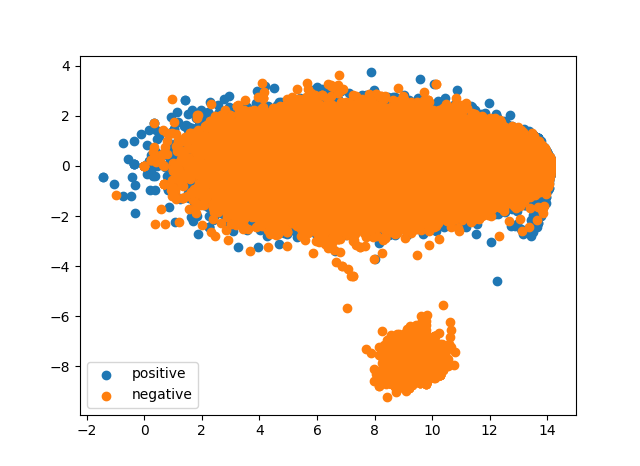
\includegraphics[width=\columnwidth]{imgs/glove_plot.png}
  \caption{Spread of tweets when representing them as the average over all their words' GloVe embeddings.}
  \label{fig:glove-embeddings}
\end{figure}

If we could come up with a way to aggregate the word vectors in such a way that the positive and negative tweets are clearly separable, we would be done. Unfortunately, coming up with one such way is far from trivial.

Much easier is to have a program \textit{learn} on itself what the embeddings should be and how they need be interpreted to allow the best predictions. This is where the convolutional neural network from \autoref{sub:cnn} comes into play. Although it is a bit trickier to implement, training is really easy, amounting to little more than throwing tweets at it, and the results are remarkable.

\todoThis{Add stuff about our novel idea.}

\todoThis{Discuss the strengths and weaknesses of your
  approach, based on the results. Point out the implications of your
  novel idea on the application concerned.}
  
\todoThis{You compare your novel algorithm to \emph{at least two baseline
  algorithms}. For the baselines, you can use the implementations you
developed as part of the programming assignments.\\}
  
\section{Summary}\label{sec:summary}
\todoThis{Summarize your contributions in light of the new
  results.}

\section*{Acknowledgements}
\todo

or remove section if none

\bibliographystyle{IEEEtran}
\bibliography{report}
\section{(DELETE before submission)}
\todoThis{Remove this section before submission}\\

Your semester project is a group effort. It consists of four parts:
\begin{enumerate}
\item The programming assignments you solve during the semester.
\item Developing a novel solution for one of the assignments, e.g. by
  combining methods from previous programming assignments into a novel
  solution.
\item Comparing your novel solution to previous assignments.
\item Writing up your findings in a short scientific paper.
\end{enumerate}

There are two different types of grading criteria applied to your
project, with the corresponding weights shown in brackets.
\begin{description}
\item[Competitive] \ \\
  The following criteria is scored based on your rank
  in comparison with the rest of the class.
  \begin{itemize}
  \item time taken for computation (10\%)
  \item average rank for all other criteria relevant to the task, for
    example reconstruction error and sparsity (20\%)
  \end{itemize}
  The ranks will then be converted on a linear scale into a grade
  between 4 and 6.
\item[Non-competitive] \ \\
  The following criteria is scored based on an
  evaluation by the teaching assistants.
  \begin{itemize}
  \item quality of paper (30\%)
  \item quality of implementation (20\%)
  \item creativity of solution (20\%)
  \end{itemize}
\end{description}

\textcolor{red}{The document should be a maximum of {\bf 4 pages}.}\\

As for code...
\begin{itemize}
\item Have a \texttt{README} file that (at least) describes what your
  software does, and which commands to run to obtain results. Also
  mention anything special that needs to be set up, such as
  toolboxes\footnote{For those who are
  particularly interested, other common structures can be found at
  \url{http://en.wikipedia.org/wiki/README} and
  \url{http://www.gnu.org/software/womb/gnits/}.}.
\item A list of authors and contributors can be included in a file
  called \texttt{AUTHORS}, acknowledging any help that you may have
  obtained. For small projects, this information is often also
  included in the \texttt{README}.
\item Use meaningful filenames, and not \texttt{temp1.m},
  \texttt{temp2.m}. The code should also unzip into a subdirectory.
\item Document your code. Each file should at least have a short
  description about its reason for existence. Non obvious steps in the
  code should be commented.
\item Describe how the results presented in your paper can potentially
  be reproduced.
\end{itemize}
\end{document}
